\documentclass[11pt]{report}

%%METADATA
\title{Notes on Trade, Macro, Spatial, and IO}
\author{
Junbiao Chen\thanks{E-mail: junbiaochen1998@gmail.com.
All errors are my own.}
}
\date{}

%%PACKAGES
\usepackage{graphicx}
\usepackage{grffile}
\graphicspath{ {../output/figures/} }
\usepackage{tabularx}
\usepackage{setspace}
\usepackage{amsmath,amsthm,amssymb}
\usepackage[hyphens]{url}
\usepackage{natbib}
\usepackage[font=normalsize,labelfont=bf]{caption}
\usepackage[margin=1in]{geometry}
\usepackage{hyperref}
\hypersetup{colorlinks=true,urlcolor=blue,citecolor=blue}
\usepackage{stmaryrd}  %Package with \boxast command
\usepackage{enumerate}% http://ctan.org/pkg/enumerate %Supports lowercase Roman-letter enumeration
\usepackage{verbatim} %Package with \begin{comment} environment
%\usepackage{enumitem}
\usepackage{physics}
\usepackage{tikz}
\usepackage{listings}
\usepackage{upquote}
\usepackage{booktabs} %Package with \toprule and \bottomrule
\usepackage{etoc}     %Package with \localtableofcontents
\usepackage{placeins}    %Package that prevent repositioning the tables
\usepackage{multicol}
\usepackage{bm}
\usepackage{subfig}
\usepackage{csquotes}

\definecolor{dkgreen}{rgb}{0,0.6,0}
\definecolor{gray}{rgb}{0.5,0.5,0.5}
\definecolor{mauve}{rgb}{0.58,0,0.82}

\lstset{language=bash,
  frame=tb,
  aboveskip=3mm,
  belowskip=3mm,
  showstringspaces=false,
  columns=flexible,
  basicstyle={\small\ttfamily},
  numbers=none,
  numberstyle=\tiny\color{gray},
  keywordstyle=\color{blue},
  commentstyle=\color{dkgreen},
  stringstyle=\color{mauve},
  breaklines=true,
  breakatwhitespace=false,
  tabsize=3
}

\lstset{language=C,
  aboveskip=3mm,
  belowskip=3mm,
  showstringspaces=false,
  columns=flexible,
  basicstyle={\small\ttfamily},
  numbers=none,
  numberstyle=\tiny\color{gray},
  keywordstyle=\color{blue},
  commentstyle=\color{dkgreen},
  stringstyle=\color{mauve},
  breaklines=true,
  breakatwhitespace=false,
  tabsize=4
}

%CUSTOM DEFINITIONS
\theoremstyle{definition}
\newtheorem{definition}{Definition}[section]
\newtheorem*{remark}{Remark}
\setcounter{secnumdepth}{3}
\usepackage{tikz}
\usetikzlibrary{automata, positioning, arrows, calc}

\tikzset{
	->,  % makes the edges directed
	>=stealth, % makes the arrow heads bold
	shorten >=2pt, shorten <=2pt, % shorten the arrow
	node distance=3cm, % specifies the minimum distance between two nodes. Change if n
	every state/.style={draw=blue!55,very thick,fill=blue!20}, % sets the properties for each ’state’ n
	initial text=$ $, % sets the text that appears on the start arrow
 }

%%FORMATTING
\onehalfspacing
\numberwithin{equation}{section}
\numberwithin{figure}{section}
\numberwithin{table}{section}
\bibliographystyle{../bib/aeanobold-oxford}

%LOGBOOK
\begin{document}

%%LOGBOOK COVER
\maketitle

%TABLE OF CONTENTS
\renewcommand{\thechapter}{\Alph{chapter}}
\setcounter{tocdepth}{2}
\tableofcontents
\etocsettocstyle{}{} % from now on only local tocs

\chapter{Spatial Economics}
\section{Spatial Equilibrium}
\subsection{``On the Equilibrium Properties of Spatial Models'' \\ \citep{Allen:2024}}  \subsubsection{Setting}
Exponential growth in computational power and new micro-data allow
the empirical implementation of models where large number of agents (e.g., locations) interact 
with each other in multiple ways (e.g., spatial linkages).

Consider a system of $N$ locations across which there are $H$ types of interactions whose equilibrium 
can be reduced to a set of $N \times H$ equations of the following forms:
\begin{equation}
    \label{eqn:AAL_NH_system}
    x_{ih} = \sum_{j = 1}^N f_{ijh}(x_{j1}, x_{j2}, \cdots, x_{jH})
\end{equation}
where $\{ x_{ih}\} \in \mathbb{R}_{++}^{N \times H}$ reflect the (strictly positive) equilibrium outcome
of each interaction in each locations,
and $f_{ijh}: \mathbb{R}_{++}^{H} \rightarrow \mathbb{R}_{++}$ are known functions that govern the interactions across locations.
In other words, $f_{ijh}$ governs the impact of location $j$ on $i$'s $h$ via $H$ linkages.

\subsubsection{Overview}
This paper provides a new theorem that offers
\begin{enumerate}
    \item an iterative algorithm for calculating an equilibrium and 
    \item sufficient and “globally necessary” conditions under which the equilibrium is unique.
\end{enumerate}
In short, this paper approaches the analysis of $N^2 \times H$ functions $\{ f_{ijh} \}$ in equation~(\ref{eqn:AAL_NH_system})
to a $H \times H$ matrix $(\mathbf{A})_{hh'} \equiv \sup_{ij} \left( \mid \frac{\partial \ln f_{ijh}}{\partial \ln x_{jh'}} \mid \right)$
that characterize the strength of the economic interactions.

\subsubsection{Perov Fixed Point Theorem}
Let $\left\{\left(X_h, d_h\right)\right\}_{h=1,2, \ldots, H}$ be $H$ metric spaces 
where $X_h$ is a set and $d_h$ is its corresponding metric. 
Define $X \equiv X_1 \times X_2 \times \ldots \times X_H$, 
and $d$ : $X \times X \rightarrow \mathbb{R}_{+}^H$ such that 
for $x=\left(x_{1, \ldots,} x_H\right)$, 
$x^{\prime}=\left(x_{1, \ldots,}^{\prime}, x_H^{\prime}\right) \in X$, 
$d\left(x, x^{\prime}\right)=\left(\begin{array}{c}d_1\left(x_1, x_1^{\prime}\right) \\ \ldots \\ d_H\left(x_H, x_H^{\prime}\right)\end{array}\right)$. 
Given operator $T: X \rightarrow X$, suppose for any $x, x^{\prime} \in X$
$$
d\left(T(x), T\left(x^{\prime}\right)\right) \leq \mathbf{A} d\left(x, x^{\prime}\right)
$$
where $\mathbf{A}$ is a non-negative matrix and the inequality is entry-wise. 
Denote $\rho \mathbf{( \mathbf { A } ) \text { as the }}$ spectral radius of $\mathbf{A}$. If $\rho(\mathbf{A})<1$ 
and for all $h=1,2, \ldots, H,\left(X_h, d_h\right)$ is complete, 
there exists a unique fixed point of $T$, 
and for any $x \in X$, the sequence of $x, T(x), T(T(x)), \ldots$ 
converges to the fixed point of $T$.

\subsubsection{The Theorem}

\begin{table}[h]
    \caption{Notations in \cite{Allen:2024}}
        \centering
        \begin{tabular}{c l} \toprule
            Notation & Meaning \\ \hline
            $f_{ijh}$ & type $h$-spatial linkage \\
            $x_{ih}$ & location $i$'s equilibrium outcome $h$ \\
            $\epsilon_{ijh,jh'}(x_{j})$ & the impact of location $j$'s outcome $h'$ on $i$'s outcome h \\
            $\mathbf{A}$ & bounds of the elasticities $\epsilon_{ijh,jh'}(x_{j})$ \\
            $\rho(\mathbf{A})$ & spectral radius of matrix $\mathbf{A}$ \\
            \bottomrule
        \end{tabular}
        \begin{minipage}{0.6\textwidth}{\footnotesize
            \textsc{Notes}:}
        \end{minipage}
\end{table}

\paragraph{Theorem 1}
Suppose there exists an $H$-by-$H$ matrix $\mathbf{A}$ 
such that for all $i, j \in \mathcal{N}, h, h^{\prime} \in \mathcal{H}$, 
and $x_j \in \mathbb{R}_{++}^H,\left|\epsilon_{i j h, j h^{\prime}}\left(x_j\right)\right| \leq(\mathbf{A})_{h h^{\prime}}$. 
Then:
\begin{enumerate}[(i)]
    \item If $\rho(\mathbf{A})<1$, then there exists a unique solution to equation (1) which can be computed by iteratively applying equation (1) with a rate of convergence $\rho \mathbf{( A )}$;
    \item If $\rho(\mathbf{A})=1$ and:
    a. For all $i \in \mathcal{N}$ and $h, h^{\prime} \in \mathcal{H}$ when $(\mathbf{A})_{h h^{\prime}} \neq 0$ there exists some $j$ such that for all $x_j \in \mathbb{R}_{++}^H,\left|\epsilon_{i j h, j h^{\prime}}\left(x_j\right)\right|<(\mathbf{A})_{h h^{\prime}}$, then equation (1) has at most one solution;
    b. For all $x_j, \epsilon_{i j h, j h^{\prime}}\left(x_j\right)=\alpha_{h h^{\prime}} \in \mathbb{R}$ where $\left|\alpha_{h h^{\prime}}\right|=(\mathbf{A})_{h h^{\prime}}$ for all $i, j \in \mathcal{N}$ and $h, h^{\prime} \in$ $\mathcal{H}$-i.e. $f_{i j h}\left(x_j\right)=K_{i j h} \prod_{h^{\prime} \in \mathcal{H}} x_{j h^{\prime}}^{\alpha_{h h^{\prime}}}$ for some $K_{i j h}>0$-then there is at most one columnwise up-to-scale solution, i.e. for every two solutions $x$ and $x^{\prime}$ and $h \in \mathcal{H}$, it must be $x_{. h}^{\prime}=c_h x_{. h}$ for some scalar $c_h>0$;
    \item If $\rho(\mathbf{A})>1$ and $N \geq 2 H+1$, then there exists some $\left\{K_{i j h}>0\right\}_{i, j \in \mathcal{N}, h \in \mathcal{H}}$ such that for $f_{i j h}\left(x_j\right)=K_{i j h} \prod_{h^{\prime} \in \mathcal{H}} x_{j h^{\prime}}^{\alpha_{h h^{\prime}}}$ where $\alpha_{h h^{\prime}} \in \mathbb{R}$ and $\left|\alpha_{h h^{\prime}}\right|=(\mathbf{A})_{h h^{\prime}}$, equation (1) has multiple solutions that are column-wise up-to-scale different, i.e. it has two solutions $x$ and $x^{\prime}$ such that for some $h \in \mathcal{H}, x_{. h}^{\prime} \neq c_h x_{. h}$ with every $c_h>0$.
    
\end{enumerate}

Proof. Part (i): Notice that equation~(\ref{eqn:AAL_NH_system}) 
can be written as 
$y_{i h} \equiv \ln x_{i h}=\ln \sum_{j \in \mathcal{N}} f_{i j h}\left(\exp \ln x_j\right)$ 
and furthermore denote its right side as function $g_{i h}(y)$ for matrix $y$, we thus have:
\begin{equation}
    \label{eqn:proof_part_i1}
    \frac{\partial g_{i h}}{\partial y_{j h^{\prime}}}=\frac{\epsilon_{i j h, j h^{\prime}}\left(\exp y_j\right) f_{i j h}\left(\exp y_j\right)}{\sum_{k \in \mathcal{N}} f_{i k h}\left(\exp y_j\right)}
\end{equation}



Given any $y$ and $y^{\prime}$, according to the mean value theorem, for each $i$ and $h$, 
there exists $\hat{y}=\left(1-t_{i h}\right) y+t_{i h} y^{\prime}$ where $t_{i h} \in[0,1]$ such that:
\begin{equation}
    \label{eqn:proof_part_i2}
    g_{i h}(y)-g_{i h}\left(y^{\prime}\right)=\sum_{j \in \mathcal{N}, h^{\prime} \in \mathcal{H}} \frac{\partial g_{i h}(\hat{y})}{\partial y_{j h^{\prime}}}\left(y_{j h^{\prime}}-y_{j h^{\prime}}^{\prime}\right)
\end{equation}


Equations~(\ref{eqn:proof_part_i1}) and (\ref{eqn:proof_part_i2}) together with 
condition $\left|\epsilon_{i j h, j h^{\prime}}\left(x_j\right)\right| \leq(\mathbf{A})_{h h^{\prime}}$, imply
\begin{equation}
    \label{eqn:proof_part_i3}
\left|g_{i h}(y)-g_{i h}\left(y^{\prime}\right)\right| \leq \sum_{h^{\prime} \in \mathcal{H}}(\mathbf{A})_{h h^{\prime}} \max _{j \in \mathcal{N}}\left|y_{j h^{\prime}}-y_{j h^{\prime}}^{\prime}\right|
\end{equation}

For any $h \in H$, define metric $d_h\left(y_h, y_h^{\prime}\right)=\max _{j \in \mathcal{N}}\left|y_{j h}-y_{j h}^{\prime}\right|$ on space $Y_h \equiv \mathbb{R}^N$. 
Furthermore, define $Y=Y_1 \times \ldots \times Y_H$ and $d\left(y, y^{\prime}\right)=\left[d_1\left(y_1, y_1^{\prime}\right), \ldots, d_H\left(y_H, y_H^{\prime}\right)\right]^{\prime}$ for $y, y^{\prime} \in Y$.
Notice that inequality~(\ref{eqn:proof_part_i3}) then becomes $d\left(g(y), g\left(y^{\prime}\right)\right) \leqq \mathbf{A} d\left(y, y^{\prime}\right)$. 
Thus we can apply the Perov Fixed Point Theorem to obtain the desired results 
(existence, uniqueness and computation).

\subsection{Application to Spatial Models with Input-output Linkages}

\clearpage
\section{Static Models}
\subsection{``The Impact of Regional and Sectoral Productivity Changes on the US Economy'' \citep{Caliendo:2018}}
\clearpage
\section{Dynamic Models}

\section{Spatial Growth}
\section{Optimal Spatial Policy}
\section{Transportation Networks}

%%LOGBOOK ENTRIES: Research design
\chapter{International Trade}
\section{Multi-country, Multi-sectoral Ricardian Model}
\subsection{``Estimates of the Trade and Welfare Effects of NAFTA'' \\ \citep{Caliendo:2015}} \subsubsection{Model}
The Caliendo-Parro model is a multi-industry extension of the EK (2002) Ricardian model of trade \citep{Antras:2022}.
\paragraph{Environment}
$N$ countries.
$J$ sectors.
One factor of production, labor.
CRS production function.
Output produced in all sectors can be used as intermediate input or a final good.

\paragraph{Preferences}
The representative consumer in each country has preferences over the output of the $S$ sectors given by:
\begin{equation}
    u(C_n) = \prod_{j=1}^J \left(C_n^j \right)^{\alpha_j}, \quad \text{where } \sum_{j} \alpha_j = 1
\end{equation}
where $C_n^j$ denotes non-tradable a final (consumer) good.%
\footnote{
    \cite{Antras:2022} refer $C_n^j$ as a consumer good.
}

\begin{figure}[h!]
    \centering
    \caption{Roundabout Production}
    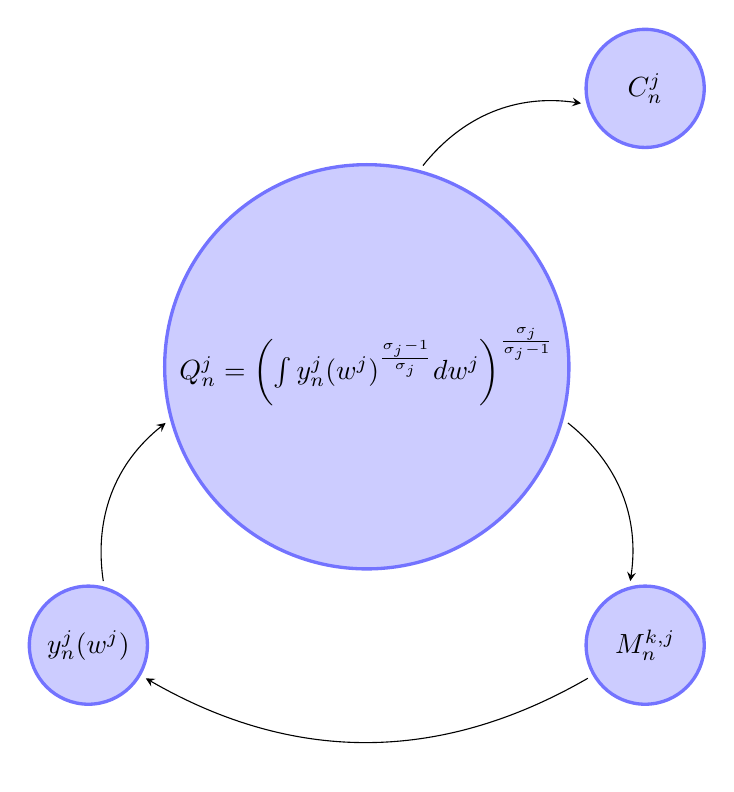
\begin{tikzpicture}[node distance=50mm, on grid]
        % Nodes arranged in a circular layout
        \node[state, minimum size=32mm] (Q) 
            {$Q_n^j = \left(\int y_n^j (w^j)^{\frac{\sigma_j-1}{\sigma_j}} d w^j \right)^{\frac{\sigma_j}{\sigma_j - 1}}$};
        \node[state, minimum size=15mm, above right=of Q] (C) {$C_n^j$};
        \node[state, minimum size=15mm, below right=of Q] (M) {$M_n^{k,j}$};
        \node[state, minimum size=15mm, below left=of Q] (y) {$y_n^j(w^j)$};
        
        % Edges to represent the roundabout process
        \draw[->, bend left] (Q) to (C);
        \draw[->, bend left] (Q) to (M);
        \draw[->, bend left] (M) to (y);
        \draw[->, bend left] (y) to (Q);
    \end{tikzpicture}
\end{figure}

\paragraph{Intermediate goods}%
\footnote{
    \cite{Antras:2022} term the production function in \cite{Caliendo:2015} as a ``roundabout model''
    and suggest that ``it has quickly become a benchmark model in the field [of modeling GVCs with macro approaches].
    The macro approaches emphasize the role of trade in intermediate inputs and of global inter-sectoral linkages 
    in shaping response of the world economy to various types of shocks.''
}
A continuum of intermediate goods $\omega^j \in [0, 1]$ is produced in each sector $j$.
Two types of inputs, labor and ``materials from all sectors'' are used for the 
production of each $\omega^j$.
The production technology of a good $\omega^j$ is 
\begin{equation}
    y_n^j(w^j) = z_n^j(w^j)\bigg[ l_n^j(w^j) \bigg]^{\gamma_n^j} \prod_{k=1}^J \bigg[ M_n^{k,j}(w^j) \bigg]^{\gamma_n^{k,j}}
\end{equation}
where
\begin{enumerate}
    \item $z_n^j(w^j) \sim \text{Frechet}$ governs the efficiency of producing intermediate good $\omega^j$ in county $n$
    \item $l_n^j(w^j)$ is labor
    \item $M_n^{k,j}(w^j)$ is the materials from sector $k$ used for the production of intermediate good $\omega^j$ (capturing the roundabout production)
    \item $\gamma_n^{k,j} \geq 0$ is the share of the materials used from $k$ in $j$ (capturing the strength of the I-O linkages)
\end{enumerate}

\paragraph{Composite goods}%
Producers of composite goods in sector $j$ and country $n$, supply final consumptions $C_n^j$ and materials $M_n^{k,j}$

\section{Multinational Production}
In this section, I summarize the multinational production literature that 
explicitly model the role of platform by multinational firms.%
% \footnote{
% This section is largely based on Felix Tintelnot's lecture notes.
% }
These flows are important because 
\begin{enumerate}
    \item A large share of foreign affiliates' production is exported to other countries, beyond exports back to their parent countries \citep{Tintelnot:2017}.
    \item They also lead to interesting implications for commercial policy and for the welfare gains from trade and multinational production.
\end{enumerate}

The main challenge for modeling export platforms is the ugly corner solutions for production, consumption, and trade.
However, it is not surprising that,
the same solution that EK (2002) provided for extending the Ricardian trade model to multiple countries is 
also helpful for the extension of the multinational production models to multiple countries:
\textbf{A probabilistic structure based on the Frechet distribution.}
\begin{equation}
    \text{Pr}( Z_i(j) \leq z) = F_i(z) = \exp(-T_i z^{-\theta})
\end{equation}
where 
\begin{itemize}
    \item $T_i > 0$ governs the \textbf{location} of $F_i(z)$. 
Higher $T_i$ implies higher productivity draw is more likely for any good $j$. ``Absolute advantage.''
    \item $\theta > 1$ determines the dispersion of productivity, where a higher $\theta$ means there is less dispersion (common across countries).
``Comparative advantage.''
\end{itemize}

\subsection{``Trade, Multinational Production, and the Gains from Openness'' \\ \citep{Ramondo:2013}} 
\paragraph{Motivation}
The existing literature on the gains from inter-country interactions studies 
\textbf{trade in goods}, and \textbf{MP/FDI} in isolation.
The omission of combining these two interactions in analysis is important because 
trade agreements often combine tariff reductions and removal of barriers to MP.

\paragraph{Some Notations}
\begin{table}[h]
    \caption{Notations in \citep{Ramondo:2013}}
        \centering
        \begin{tabular}{c l} \toprule
            Notation & Meaning \\ \hline
            $i = \{1, 2, 3, \cdots, I\}$ & country of headquarter (parent) \\
            $l = \{1, 2, 3, \cdots, I\}$ & country of production \\
            $n = \{1, 2, 3, \cdots, I\}$ & country of destination \\
            $d_{nl} \geq 1$ & trade costs \\
            $h_{li}^g \geq 1$ & MP costs \\
            $v \in [0, 1]$ & tradable intermediate goods \\
            $u \in [0, 1]$ & non-tradable final goods \\ 
            \bottomrule
        \end{tabular}
        \begin{minipage}{0.6\textwidth}{\footnotesize
            \textsc{Notes}: $h_{li}^g \geq 1$ implies that home production is more efficient that those of foreign affiliates.}
        \end{minipage}
\end{table}


\subsubsection{Model}
\paragraph{MP Cost}
Unit cost of the MP input bundle for MP by $i$ in $l$:
\begin{equation}
 c_{li} = \bigg[ (1-a) (c_l h_{li})^{1 - \xi} + (a) (c_i d_{li})^{1 - \xi}
    \bigg]^{\frac{1}{1-\xi}}
\end{equation}

\paragraph{Productivity Distributions}
For a home country, she faces
a vector $\mathbf{z}_i^s = (z_{1i}, z_{2i}, \cdots z_{Ii}), s = g, f$ that is 
drawn independently across goods and countries from a Multivariate Frechet distribution:
\begin{equation}
    F_i\left(\mathbf{z}_i^s; T_i \right) 
    =\exp \left[-T_i\left(\sum_{l=1}^I\left(z_{l i}^s\right)^{\frac{-\theta}{1-\rho}}\right)^{1-\rho}\right]
\end{equation}
where $\rho$ governs the correlation of productivity across production locations.

\paragraph{Equilibrium Analysis}
Final goods are non-tradable, so $i$ must produce them in destination country $n$ to obtain positive market share.
Therefore, the price of final good $u$ in $n$ is 
\begin{equation*}
    p_n^f(u) = \min_i \frac{c_{ni}^f}{z_{ni}^f}
\end{equation*}

As $z_{ni}^f \sim F(z)$, 
the share of expenditure by country $n$ on final goods produced in country $n$ with country $i$ technologies is 
\begin{equation}
    \pi_{ni}^f = \frac{T_i (c_{ni}^f)^{-\theta}}{\sum_j T_j (c_{nj}^f)^{-\theta}}
\end{equation}


Compared to non-tradable final goods,
intermediate goods are tradable and can be imported from production countries that might differ 
from the home countries and destination countries $(i \neq l \neq n)$.

The price of intermediate good $v$ in $n$ is 
\begin{equation*}
    p_n^g(v) = \min_{i,l} \frac{c_{ni}^g d_{nl}}{z_{li}^g}, \quad d_{nl} \geq 1
\end{equation*}
where $z_{li}^g$ is home-production technology.
As $z_{li}^g \sim F(z)$, 
the share of expenditures by country $n$ on intermediate goods produced in country $l$ with country $i$ technology is:
\begin{equation}
    \pi_{n l i}^g = \frac{T_i\left(\tilde{c}_{n i}^g\right)^{-\theta}
            }{
                \sum_j T_j\left(\tilde{c}_{n j}^g\right)^{-\theta}} 
                \frac{\left(c_{l i}^g d_{n l}\right)^{-\theta /(1-\rho)}
                }{\sum_k\left(c_{k i}^g d_{n k}\right)^{-\theta /(1-\rho)}
                }
\end{equation}
where $\tilde{c}_{n i}^g=\left(\sum_k\left(c_{k i}^g d_{n k}\right)^{-\theta /(1-\rho)}\right)^{-(1-\rho) / \theta}$
This expression has a natural interpretation: 
The first term on the right-hand side is the share of expenditures that country $n$ allocates to intermediate goods produced with
country $i$’s technologies independently of the location where they are produced,
while the second term on the right-hand side is the share of these goods that are produced in country $l$. 

\subsubsection{Calibration}


\chapter{Econometrics}
\section{Shfit-Share Designs}
\subsection{``A Practical Guide to Shift-Share Instruments'' \\ \citep{Borusyak:2024}} A recent econometric literature shows two distinct paths for identification with shift-share instruments, 
leveraging either many exogenous shifts \citep{Borusyak:2022, Adao:2019} 
or exogenous shares \citep{Goldsmith-Pinkham:2020}. 

This paper presents the core logic of both paths and practical takeaways.


\subsection{ADH (2003)'s SSIV}
The influential China shock paper by ADH 
constructs an instrumental variable with a shift-share structure:
\begin{equation}
    \text{SSIV}_{i} = \sum_{k} \text{emp share}_{i,k} \times \text{avg. of growth in Chinese import among non-US countries}_{k}
\end{equation}
where $k$ denotes industry and $j$ denotes commuting zone.

\subsection{Definition of SSIV}
A shift-share structure follows
\begin{equation}
    z_i = \sum_{k=1}^K \underbrace{s_{ik}}_{\text{Share}} 
        \underbrace{g_k}_{\text{Shift}}
\end{equation}
\paragraph{Remarks}
\begin{itemize}
    \item Shifts vary at a different level (e.g.~industries) than the unit of analysis (e.g.~local labor markets).
    \item Shares vary across units but are usually predetermined (e.g., employment shares are measured in a pre-period).
    \item To argue convincingly that SSIV are exogenous, 
    one must explain what properties of the shifts and shares make $z_i$ uncorrelated with $\epsilon_i$ 
    (rather than simply stating $\text{Cov}[z_i, \epsilon_i]$ = 0).
    \item $\sum_{k=1}^K s_{ik}$ is generally one. For incomplete share see Section~\ref{sec:ssiv_incomplete_share}.
\end{itemize}

One strategy to ensure that the shift-share instrument $z_i$ is exogenous is to have exogenous shift $g_k$.
The key threat to identification in the exogenous shifts approach is the violation of the following condition:
\textbf{
    $g_k$ should be uncorrelated with an average of $\epsilon_i$ taken across units with weights $s_{ik}$.
}

\subsection{Incomplete Shift Share}
\label{sec:ssiv_incomplete_share}
In shift-share designs where the exposure shares $s_{i,k}$ do not add up to one,
a special control must by included: the sum of shares, $S_i = \sum_{k} s_{i,k}$.
This control remedies the bias arising from the correlation between $S_i$ and the error.

\subsection{A Checklist for the Shift-Based Approach}
\begin{enumerate}
    \item Thinking about what endogeneity bias is being addressed.
    \item Bridge the gap between the observed and ideal shifts. 
    Control for $\sum_{k} s_{ik} q_k$: shift-share aggregates of the industry-level confounders
    \item Include the ``incomplete share" control.
    \item Lag shares to the beginning of the natural experiment.
    \item Report descriptive statistics for shifts, such as mean and std.~of $z_i$ and $g_k$.
    \item Implement balance tests for shifts in addition to the instrument.
    \item Use correct standard errors.
\end{enumerate}







\chapter{Computational Economics}


\bibliography{../bib/notes.bib}

\end{document}